\documentclass{article}
\usepackage{graphicx}
\usepackage{amssymb}
\usepackage{mathtools}
\usepackage{amsmath}
\usepackage{physics}
\usepackage{authblk}
\usepackage{comment}
% Required for inserting images
\graphicspath{{images/}}
\usepackage{changepage}
\usepackage{float}
\DeclareMathOperator*{\argmin}{argmin}
\begin{document}

\title{\textbf{Popularity Prediction of Spotify Tracks}}
\author{Luca Bellani}
\author{Andrea Longoni}
\affil{Statistical Methods for Machine Learning}
\date{}

\maketitle

% \tableofcontents

\begin{abstract}
	In this paper we develop a prediction system that estimates the popularity of a song. The flow of this work starts with the manipulation of the dataset: ''Spotify Track Dataset''. The training and estimation parts, together with k-fold nested cross validation and kernel functions, are developed from scratch and compared with the \texttt{scikit-learn} operations. 
\end{abstract}
    

\section{Introduction}
Ridge Regression is a linear prediction where vectors of real coefficients are approximated by an hyperparameter called ''regularizer''. This choice is especially useful in a situation in which the training set is perturbed, thus achieving a more stable predictor for reducing the variance of the risk. \newline
In order to get the best hyperparameter $\alpha$, the k-fold nested cross validation process is built.

K-Fold Nested Cross Validation splits the dataset in $K$ parts and computes the estimate by dividing further the training data, iterates on the set of hyperparameters for each fold predictor and delivers in the end the average of their performance as output.  
For experimental purpose, we have implemented an additional part: the kernel trick. This allows us to deal with higher dimensional space data, without the explicit necessity of calculating it. In fact, this process would be computationally expensive for higher-dimensional spaces.\newline
    
The aim of this project is to analyze these different techniques in order to predict the popularity of tracks, with the purpose of determining which models and hyperparameters fit better. 
     
    
\section{Dataset}
''Spotify Track Dataset'' is a CSV dataset of Spotify tracks over a range of 125 different genres. The data was collected and cleaned using Spotify's Web API and Python. Each track has some audio features associated with it, both numerical and categorical, with a total number of 21 features that describe exactly 114000 datapoints \cite{datasetKaggle}. 

\subsection{Feature Description}
\label{subsec:feature_descr}
The attributes of the dataset represent the inertial aspects of the tracks: most of the numerical features, like \texttt{instrumentalness}, \texttt{liveness} or \texttt{speechiness}, detect the presence of the characteristics they specify, indicating the probability of how much the phenomenon occurs. 
%some of the data we have discarted
The categorical metadata show for the majority nominal characteristics: in fact, \texttt{track\_id}, \texttt{artists}, \texttt{album\_name}, \texttt{track\_name} labels are not functional and discarded from the \texttt{DataFrame} for discovering the popularity of a track. Features such as \texttt{key}, \texttt{mode} and \texttt{time\_signature} are represented as numbers but they can be considered as categorical, since are labels mapped to integer values.  

\subsection{Data Manipulation}
\label{subsec:dataman}    
The first step is to convert the \texttt{.csv} document into a \texttt{DataFrame} object. 
%data ordered by genre
The issue of the Spotify Track Dataset is that the rows are ordered alphabetically by musical genre: after we have read the file, a randomization of the datapoint position is applied, in order to enhance the prediction perfomance. Another correlated problem is that some rows are perfectly equal except for the \texttt{track\_genre} attribute: the solution is explained in the subsection \ref{subsec:track_genre}. 
%train test with mask
    
NumPy and Pandas libraries are imported for  their data structure and functions they offer, in particular for the data management and calculus.
    
Next, the data are divided randomly into two sets, training (70\%) and test (30\%).
%some of the numerical data are treated like categorical
The project focuses on training both numerical and all features, so we have momentarily dropped the categorical metadata for the first part and, as already mentioned in the section above, \texttt{key}, \texttt{mode} and \texttt{time\_signature} too. 
For a more accurate analysis, we have randomized the row positions in three distinct modes, this simply by using different seed generations. In this way we can view how much variance occurs in the estimations.


\subsection{Manage a unique track with multiple genres}
\label{subsec:track_genre}
One noticeable thing that shows up in the information set is that there are more rows with the same \texttt{track\_id} (this can be seen as a primary key) that perfectly match except for their \texttt{track\_genre} attribute. 
The solution implemented for this particular problem is managed as follows:
\begin{enumerate}
	\item build a new \texttt{DataFrame} object with \texttt{track\_id} and \texttt{track\_genre} features, in which One-Hot Encoding procedure is applied on \texttt{track\_genre}; 
	\item group by \texttt{track\_id} and aggregate the one-hot encoded features into a single line;
	\item create a temporary \texttt{DataFrame} with all the features, except for the ''non functional features'' (cited in subsection \ref{subsec:feature_descr}) and \texttt{track\_genre};
	\item merge the temporary \texttt{DataFrame} with the ''\texttt{track\_genre DataFrame}'' through inner-join, in order to achieve the final object used for the next operations.
	              
\end{enumerate}
In general, if we have the same track with multiple genres, this will be saved as multiple lines at the beginning. This method aggregates these rows into a single one, simply by keeping $1$ in the \texttt{track\_genre} cells there were before. 
    
In this manner, we have decreased the amount of datapoints down to 89740.

\subsection{Normalization Range and One-Hot Encoding}
A \texttt{min-max} normalization procedure is applied for \texttt{loudness}, \texttt{tempo} and  \texttt{duration\_ms}, because they are the only features that are not comprised in the range 0-1.\newline
In order to compute the ridge regression on all the columns, it has been performed the \texttt{One-Hot Encoding} approach: this simply converts the categorical data into binary ones. For each non-numerical data point, a binary vector is created of length equal to the number of unique categories in the variable. Each vector has a 1 in the position corresponding to the category label and 0s in all other positions. This 1 indicates the presence of that category for that particular datapoint. The result of this process expands the number of attributes up to 146, but since that the \texttt{explicit} column is binary, we keep only the true one, thus it will be considered $1$ as explicit and $0$ not. 
In the end, an additional normalization has been utilized: we achieved a $[0,100]$ interval on all features aimed at taking the same range of \texttt{popularity.}

\section{Ridge Regression}
Linear regression is an approach in which predictors are linear functions $h: \mathbb{R}^d \rightarrow \mathbb{R}$, each parameterized by a vector $\boldsymbol{w} \in \mathbb{R}$ of real coefficients: $h(\boldsymbol{x}) = \boldsymbol{w}^\top\boldsymbol{x}$. Hence, the ERM with respect to the square loss is: \begin{equation}
w_s = \argmin_{\boldsymbol{w} \in \mathbb{R}^d}\sum_{i = 1}^m(\boldsymbol{w}^\top \boldsymbol{x}_t - y_t)^2
\end{equation}
where $m$ are the number of datapoints in a training set.
    
In a matrix context, we have a closed-form expression for the predictor (the function that we are dealing with is convex, so its gradient can vanish to $0$):
    
\begin{equation}
	\boldsymbol{w} = (S^\top S)^{-1}S^\top \boldsymbol{y}
\end{equation}
where 
\begin{itemize}
	\item $S$ is a $m \times d$ design matrix ($m$ is the number of training points and $d$ is the number of features);
	\item $S^\top S$ should be nonsingular, which means that one or more of its rows/columns are not definable as a linear combination of all or some other of its rows/columns;
	\item $\boldsymbol{y} = (y_1, \dots , y_m)$, the label vector of the training set.
\end{itemize}
    
However, when $S^\top S$ is nearly singular, the variance error could grow. In order to enhance the predictor, a regularizer $\alpha > 0$ is added for increasing the stability \cite{profrr}:

\begin{equation}
\label{rr}
	\boldsymbol{w} = (\alpha I + S^\top S)^{-1}S^\top \boldsymbol{y}
\end{equation}

%implementazione
\subsection{Implementation}
The function delegated to calculate the formula above (\texttt{ridge\_regression}) takes as arguments the hyperparameter $\alpha$ and the data to fit. Next, the \texttt{popularity} vector ($\boldsymbol{y}$) is extracted from the training set. Through $NumPy$ facilities, we have computed the hyperplane $\boldsymbol{w}$ via ridge regression and converted it into a $DataFrame$ with $Pandas$. 
With the aim of predicting and see how this model works, another two functions are written:
\texttt{predict}, which outputs the estimate, and \texttt{avg\_square\_loss}, that gives as a result the mean square error (MSE) of the hyperplane $\boldsymbol{w}$ on a given test set: 
\begin{equation}
	\label{MSE}MSE(\boldsymbol{y},\boldsymbol{\hat{y}}) = \frac{1}{m}\sum_{i = 1}^m (y_i-\hat{y}_i)^2
\end{equation}
    
where, in our case, $\hat{y}_i= \boldsymbol{w}^\top \boldsymbol{x}_i$, $\boldsymbol{w} \in \mathbb{R}^d$.
    
%risultati
\subsection{Results}
From now on, the results written in this report refer to the seed generation with number $0$.
%numerical vs all (also scikit-learn, in a objective way)
%which MSE gives
%plots
\subsubsection{Numerical features}

The MSE \eqref{MSE} calculated with the regularizer $\alpha$ set to $0$ (the standard linear regression) only on numerical features is $414.79$ with a variance of $15.86$, whereas the \texttt{scikit-learn} Ridge predictor gives a MSE of $408.01$ with a variance of $14.20$. The training and test set are manipulated as written in the subsection \ref{subsec:dataman}. In the figure \ref{rrmsenun} we have considered a set of values of $\alpha$ with its resulting square losses in the ridge regression fashion. The first plot figures the ridge prediction developed from scratch, which is compared with the second plot that represents the ridge regression model of \texttt{scikit-learn}: \texttt{sklearn.linear\_model.Ridge}. 

    
\begin{figure}[H]
	\begin{adjustwidth}{0 cm}{}
		\begin{center}
			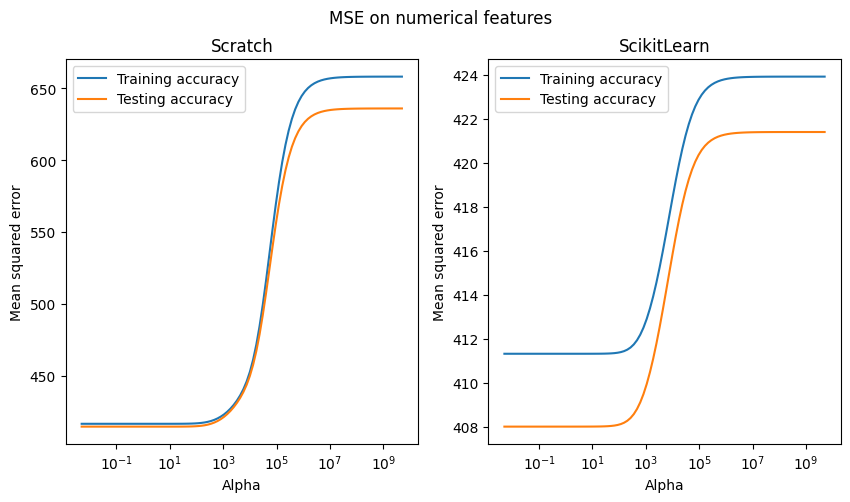
\includegraphics[scale= 0.6]{images/MSE_numerical_vs.png}
		\end{center}
	\end{adjustwidth}
	\caption{These plots depict the training and test losses, based on only numerical features in a ridge regression context. The X-Axis represents the alpha coefficients used in the estimate, while the Y-Axis represents the mean squared error given by the prediction. Note that the Y-Axis scales are different from one another.}
	\label{rrmsenun}
\end{figure}
    
\subsubsection{All features}
The MSE \eqref{MSE} calculated with the regularizer $\alpha$ set to $0$ (the standard linear regression) on all the features is $273.34$, with a variance of $31.91$, whereas the \texttt{scikit-learn} Ridge predictor gives a MSE of $273.33$ with a variance of $20.36$. The training and test set are manipulated as written in the subsection \ref{subsec:dataman}. In the figure \ref{rrmseall} we have considered a set of values of $\alpha$ with its resulting square losses in the ridge regression fashion. The first plot figures the ridge prediction developed from scratch, which is compared with the second plot that represents the ridge regression model of \texttt{scikit-learn}: \texttt{sklearn.linear\_model.Ridge}.
\begin{figure}[H]
	\begin{adjustwidth}{0 cm}{}
		\begin{center}
			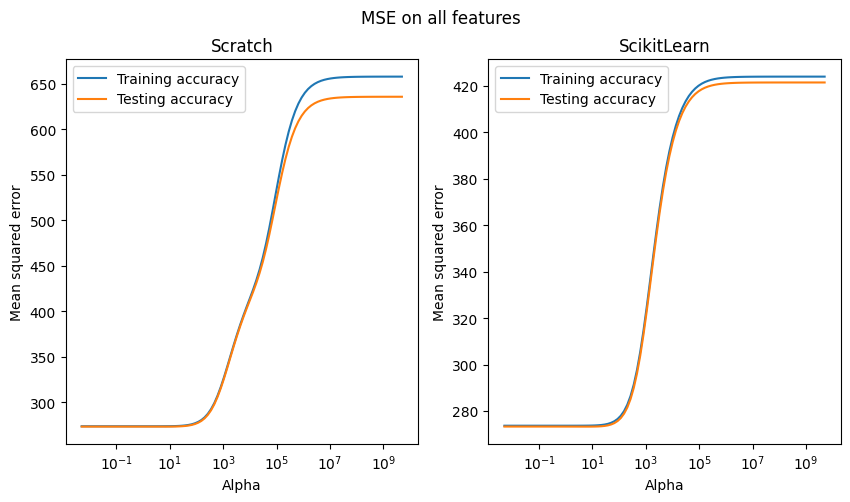
\includegraphics[scale= 0.6]{images/MSE_all_vs.png}
		\end{center}
	\end{adjustwidth}
	\caption{These plots depict the training and test losses, considering all the dataset features in a ridge regression context. The X-Axis represents the alpha coefficients, used in the estimate, while the Y-Axis represents the mean squared error given by the prediction. Note that the Y-Axis scales are different from one another.}
	\label{rrmseall}
\end{figure}

\section{K-Fold Nested Cross Validation}
Cross-validation is a technique to provide a more accurate estimate of a model's performance and to prevent overfitting. This is done by testing an entire set of hyperparameters $\Theta_0 \subset \Theta$, where $\Theta$ is the set of all possible hyperparameter values. The nested CV is an extension of traditional cross-validation and is particularly useful when you want to tune hyperparameters.
The code partitions the entire dataset $S$ in $K$ parts or folds, denoted by $i = 1,\dots,K$. The algorithm computes the loss of the correspondent predictor on the test set $S_i$ and it is executed on each training part $S_{-i} = S \setminus S_{i}$. The estimate is calculated by splitting further the training data in two subsets, $S_{train}$ and $S_{dev}$. The development set $S_{dev}$ (also called validation set) is used as a surrogate test set. The algorithm is run on $S_{train}$ once for each value of the hyperparameter in $\Theta_0$. The resulting predictors are tested on the $S_{dev}$ set. In order to obtain the final predictor, the learning algorithm is run once more on the original training set $S_{-i}$ using the value of the $\theta$ corresponding to the predictor with smallest error on the validation set. In the end, the cross validation estimate is calculated by averaging the test errors of the predictors \cite{profcv}. \newline

\subsection{Implementation}
The Nested CV method picks as input the list of the hyperparameters $alphas$, the $K$ number of folds and the dataset $S$. As mentioned above, the data are subdivided into a test set $S_{test}$ and a training set $S_{train} = S \setminus S_{test}$ for each iteration $i = 1, \dots, K$. In the nested part, we cut up $S_{train}$ in $CV_{train}$ and $CV_{dev}$ (validation set). Then, for each $alpha \in alphas$, we predict $\boldsymbol{w}$ through ridge regression \eqref{rr}. We take into account the $alpha$ that has generated the minor loss in the estimate. At the end of the external loop, a last prediction is made by taking up the entire training set and tested with $S_{test}$.
Finally, after have examined all the folds, the average of the $K$ losses is calculated and returned by the method, together with the hyperparameter $alpha$ and the best predictor $\boldsymbol{w}$. 
%what is it
%formule
%pregi
%implementazione
%risultati
\subsection{Results}
The hyperparameter tuning provides an $\alpha$ equal to $53613$, with a resulting MSE \eqref{MSE} of $275.39$. The classifier \texttt{sklearn.linear\_model.RidgeCV} delivers a MSE value of $273.35$. As shown in figure \ref{rrmseall}, the choice of $\alpha$ does not significantly affect the rate of the MSE (9) until the order of magnitude of about $10^6$.
%numerical vs all (also scikit-learn, in a objective way)
%which MSE gives
%plots

\section{Kernel Ridge Regression}
%what is it
The kernel trick facilitates the feature expansion without effectively transform data. This procedure makes us avoid an exponential computational cost of $N = \Theta(d^n)$, where $d$ is the number of features and $n$ is the number of dimensions we want to reach. In general, a kernel can be defined in this way: consider a function $\boldsymbol{\phi}: \mathbb{R}^d \rightarrow \mathcal{H}$ that maps data points on an higher feature dimensional space $\mathcal{H}$ and a general linear predictor learned through the Perceptron: \begin{equation}
h(x) = sgn\left(\sum_{s \in S}y_s\boldsymbol{x_s^\top}\boldsymbol{x}\right)
\end{equation} where $S$ is the set of indices of training examples $(\boldsymbol{x}_s,\boldsymbol{y}_s)$ on which the Perceptron made an update. In the space $\mathbb{R}^N \equiv \mathcal{H}$, the classifier becomes: \begin{equation}
h{_\phi}(x) = sgn\left(\sum_{s \in S}y_s\boldsymbol{\phi(x_s)^\top}\boldsymbol{\phi(x)}\right).
\end{equation}
    
    
The faster way to enhance the calculation speed of $\boldsymbol{\phi(x_s)^\top}\boldsymbol{\phi(x)}$ is by introducing a kernel function such that: $K(\boldsymbol{x},\boldsymbol{x^\prime}) = \boldsymbol{\phi(x)^\top}\boldsymbol{\phi(x^\prime)}.$

Some kernel functions are:
\begin{itemize}
	\item Linear Kernel: $K_1(\boldsymbol{x},\boldsymbol{x^\prime}) = \boldsymbol{x}^\top\boldsymbol{x^\prime}\hfill
	      \stepcounter{equation}\ (\theequation)$
	\item Polynomial Kernel: $K_2(\boldsymbol{x},\boldsymbol{x^\prime}) = (1 + \boldsymbol{x}^\top\boldsymbol{x^\prime})^n\hfill \stepcounter{equation}\ (\theequation)$
	\item Gaussian Kernel: 
	      $K_3(\boldsymbol{x},\boldsymbol{x^\prime}) = exp \left(-\frac{1}{2\gamma}\norm{\boldsymbol{x}-\boldsymbol{x^\prime}}^2 \right)\hfill
	      \stepcounter{equation}\ (\theequation)$
\end{itemize}
To ''kernelize'' the ridge regression predictor $\boldsymbol{w} = (\alpha I + S^\top S)^{-1}S^\top \boldsymbol{y}$, we can represent it in a generic Reproducing Kernel Hilbert Space (RKHS) \cite{rhks}: 
\begin{equation}
	\label{KRR}\langle{g,\phi_K(\boldsymbol{x})}\rangle_K = \boldsymbol{y^\top}(\alpha I + \boldsymbol{K})^{-1} \boldsymbol{k}(\boldsymbol{x})
\end{equation} 
where $K$ is the $m \times m$ matrix with entries $\boldsymbol{K}_{i,j} = K(\boldsymbol{x}_i,\boldsymbol{x}_j)$ and $\boldsymbol{k}(\boldsymbol{x})$ is the vector $(K(\boldsymbol{x}_1, \boldsymbol{x}), \dots, (K(\boldsymbol{x}_m, \boldsymbol{x}))$ of functions $K(\boldsymbol{x}_t, \boldsymbol{x}) = \langle{\phi_K(\boldsymbol{x}_t, \boldsymbol{x})}\rangle_K$ 
\cite{profk}.

\subsection{Implementation}
\label{kernelimpl}
In this project has been decided to deal with the Gaussian Kernel (9).
For experimental purpose, we have tested two possible researches for the hyperparameter $\gamma$: the cross validation and the determination of the average norm on a number of datapoints. The last solution just cited has been carried out for the reason that if $\gamma$ is relatively small to the typical euclidean squared distances between training and test points, this will imply a training error equal or close to zero, with a resulting overfitting of the predictor. At the contrary, large $\gamma$ values with respect to the euclidean squared distances cause to the resulted predictors to underfit \cite{profk}. In order to respect so, we have analyzed whether or not the investigation of the average distance of the datapoints is meaningful.\newline

\subsubsection{Kernel Functions}
\label{subsubsec:kernelfunc}
The code part for the Kernel Ridge Regression is made up of four functions:
\begin{itemize}
	\item \texttt{gaussian\_kernel}: this function takes the hyperparameter $\gamma$ and the two vectors for calculating the formula of the Gaussian Kernel (9);
	              
	\item \texttt{kernel\_ridge\_regression}: it considers as input the dataset and the hyperparameters $\alpha$ and $\gamma$. 
	      The vector $\boldsymbol{y}$ is extracted from the dataset \eqref{KRR} by taking the \texttt{popularity} column. Then, an iteration will be made in order to take the entries and calculate the matrix $\boldsymbol{K}$ \eqref{KRR}. 
	      It's observable that $\boldsymbol{K}(x_i, x_j) = \boldsymbol{K}(x_j, x_i)$ with $ i,j = 1, \dots, m$ for the square norm in the Gaussian Kernel formula (9). Hence, to halve the computation, we have calculated only the triangle above the matrix diagonal and summed it to its transpose part. Finally, we have summed the matrix $\boldsymbol{K}$ with the identity matrix scaled by $\alpha$, then we have inverted and multiplied it by the vector $\boldsymbol{y}$.
	\item \texttt{kernel\_predict}:
	      in this method we take the vector $\boldsymbol{x}$ and, examining all the training points, we determining $\boldsymbol{k}(\boldsymbol{x})$ \eqref{KRR}. In the end we obtain the estimate by factorize the \texttt{kernel\_ridge\_regression} output with $\boldsymbol{k}(\boldsymbol{x})$. 
	\item \texttt{kernel\_avg\_square\_loss}: the process of this functionality is predicting the estimate on the test set values and then calculating the MSE \eqref{MSE}.  
\end{itemize}

\subsubsection{Results}
In this section we are focusing on the values $\alpha = 1$ and $\gamma$ that is achieved by calculating, for each number of samples in table \ref{sampletable}, the average distance of the first $n$ datapoints. The considered $\gamma$ for the current analysis is the one got from $10000$ samples. The sizes of the sets are $7500$ for training and $2500$ for testing.

\begin{table}[H]
	\label{sampletable}
	\centering
	\begin{tabular}{|l|l|}
		\hline
		Samples & Average Distance   \\ \hline
		100     & $71913$ \\ \hline
		500     & $68506$ \\ \hline
		1000    & $68946$  \\ \hline
		5000    & $68477$ \\ \hline
		10000   & $68300$  \\ \hline
	\end{tabular}
\end{table}

The test made on the numerical features gives an MSE (9) of $392.38$, with a variance of $14.57$, whereas considering all the features decreases the average loss to $281.30$ with a variance of $55.32$. The \texttt{scikit-learn} predictor \texttt{KernelRidge} provides a test error of $281.31$ with a variance of $55.57$, given \texttt{RBF} as kernel function \cite{rbf}. This kernel function differs from (9) because:

\begin{equation}
    K(\boldsymbol{x},\boldsymbol{x^\prime}) = exp \left(-\frac{1}{2\gamma^2}\norm{\boldsymbol{x}-\boldsymbol{x^\prime}}^2 \right)\hfill
\end{equation}
       
The unique difference is that $\gamma$ is squared. In the test phase we have simply passed to the function the root squared average norm considered for the precedent tests.

\subsection{Kernel Cross Validation}
The hyperparameter tuning is now done on both $\gamma$ and $\alpha$. The procedure is almost the same: the only difference is that the prediction and the loss are made by the kernel functions (see section \ref{subsubsec:kernelfunc}). In order to estimate the two best hyperparameters, it has been implemented an outside loop from the nested cross validation that checks for each $\alpha$ its best $\gamma$ value. 
\subsubsection{Results}
For this topic, the hyperpameters are chosen from a set of values generated at random. The cross validation process is built with a number of $1000$ samples, due to the huge amount of computation. 
\begin{figure}[H]
	\begin{adjustwidth}{0 cm}{}
		\begin{center}
			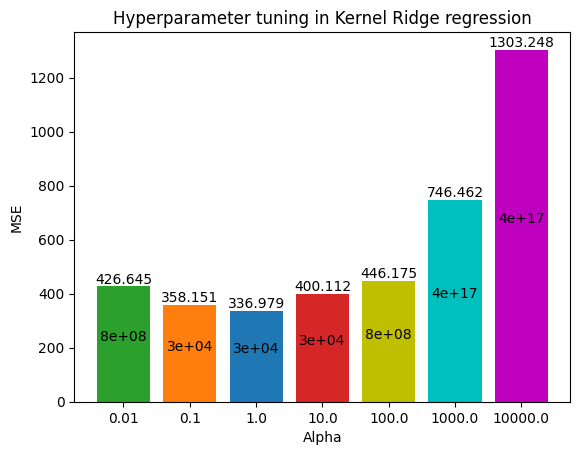
\includegraphics[scale= 0.7]{images/hyptuningKRR.png}
		\end{center}
	\end{adjustwidth}
	\caption{The histogram reveals, for each $\alpha$, the respect average square loss considering the $\gamma$ value that minimizes the MSE itself.}
	\label{hyptuningKRR}
\end{figure}
    
Once we have selected the best $\alpha$ and $\gamma$ values, we re-train the model with $7500$ datapoints and tested with $2500$. The MSE obtained is $276.14$. 
%formule
%Gaussian Kernel
%pregi
%implementazione
%risultati
%numerical vs all (also scikit-learn, in a objective way)
%which MSE gives
%Avg norm vs CV
%plots

\section{Conclusion}
%numerical vs all
The results show a sensible decrease when all the features have been considered in respect of examining only the numerical ones in the ridge regression fashion. In the figures \ref{rrmsenun} and \ref{rrmseall} it has been compared the MSE (9) considering a wide range of the hyperparameter $\alpha$, using two different ridge regression predictors. Both of them depict almost the same loss in the first $\alpha$'s orders of magnitude: in fact, when we deal with nested cross validation, the results are approximately equal, as illustrated in the figure \ref{CVscrsk}.   

    
\begin{figure}[H]
	\begin{adjustwidth}{0 cm}{}
		\begin{center}
			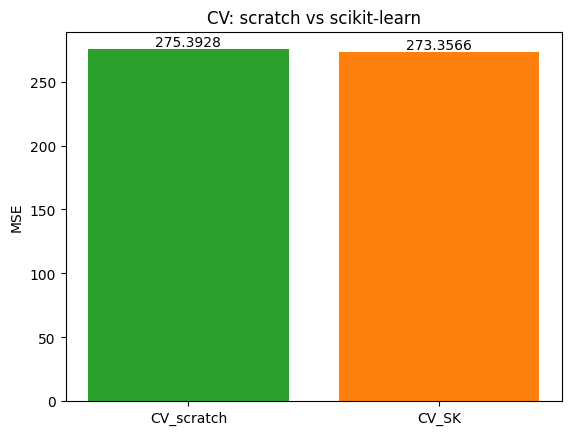
\includegraphics[scale= 0.53]{images/finalCV.png}
		\end{center}
	\end{adjustwidth}
	\caption{The histogram shows the MSEs comparison between the ridge regression model developed from scratch and \texttt{scikit-learn} ridge regressor considering all dataset features and all the datapoints.}
	\label{CVscrsk}
\end{figure}
%avg norm vs cv
The resultant values illustrated by the kernel computations in the figure \ref{KRRcomparison} do not reflect neither a significant worsening nor an improvement in terms of loss compared to the standard linear ridge prediction. Thus, it should be identical choosing one of the two models in terms of yield. However, the ridge regression predictor takes less time to compute with respect to the kernel one. In addition, in the first one we consider all of the datapoints in the estimation, which is literally inconceivable for the kernel to process. One improvement of this work could be to take into account the kernel model considering the whole dataset, in order to verify whether or not this predictor might refine its estimations. 

\begin{figure}[H]
	\begin{adjustwidth}{0 cm}{}
		\begin{center}
			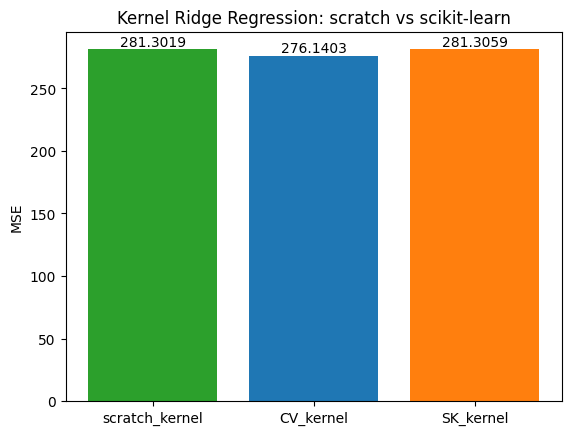
\includegraphics[scale= 0.53]{images/finalKernel.png}
		\end{center}
	\end{adjustwidth}
	\caption{The histogram shows the MSEs comparison among the kernel developed from scratch (with the average square distance), the kernel with the hyperparameters achieved by cross validation and \texttt{scikit-learn} RBF kernel \cite{rbf} considering all dataset features.}
	\label{KRRcomparison}
\end{figure}

The experiment with contemplating the average datapoint distance as the bandwith parameter of the Gaussian Kernel $\gamma$ (9) works. Indeed, as figured in the picture \ref{KRRcomparison}, the order of magnitude of the MSE value is equal to the one in which a nested cross validation is computed. This confirms what mentioned in the subsection \ref{kernelimpl}: a $\gamma$ close to the distance of the examined datapoints is an ideal rate for the predictor. 

\newpage

\bibliographystyle{unsrt}
\bibliography{biblio}

\vspace{36pt}
% \bigskip
% \bigskip
% \bigskip

\let\thefootnote\relax\footnotetext{We declare that this material, which we now submit for assessment, is entirely our own work and has not been taken from the work of others, save and to the extent that such work has been cited and acknowledged within the text of our work. We understand that plagiarism, collusion, and copying are grave and serious offences in the university and accept the penalties that would be imposed should I engage in plagiarism, collusion or copying. This assignment, or any part of it, has not been previously submitted by us or any other person for assessment on this or any other course of study.}

\end{document}
